\hypertarget{a00013}{
\section{Dokumentacja klasy ASS8.Klient.komunikacja}
\label{d7/dd4/a00013}\index{ASS8::Klient::komunikacja@{ASS8::Klient::komunikacja}}
}
\subsection*{Metody publiczne}
\begin{CompactItemize}
\item 
void \hyperlink{a00013_5069ee8ced0e023865e277f07ba690a9}{wyslij} (byte\mbox{[}$\,$\mbox{]} wiadomosc, int dlugosc)
\begin{CompactList}\small\item\em Wysyła wiadomość do serwera. \item\end{CompactList}\item 
void \hyperlink{a00013_da808f405d71a8f5f06659bac3b3fe50}{ustawUstawienia} (string s, int p)
\begin{CompactList}\small\item\em Ustawia serwer i port do połączenia. \item\end{CompactList}\item 
\hyperlink{a00013_178f432b69d8d6f2c1d6b8f6d1c43eb9}{komunikacja} ()
\begin{CompactList}\small\item\em Kontruktor klasy. \item\end{CompactList}\item 
int \hyperlink{a00013_cdc8379f1139bc25fb24a6c9b6ce1cc1}{login} ()
\begin{CompactList}\small\item\em Loguje do serwera. \item\end{CompactList}\item 
int \hyperlink{a00013_d93f81514442cd3a5eeea0db9b1c9148}{downloadFiles} (string\mbox{[}$\,$\mbox{]} nazwyPlikow, string uzytkownik, GLItem gli, string path)
\begin{CompactList}\small\item\em Ściąga \hyperlink{a00017}{pliki} z serwera. \item\end{CompactList}\item 
int \hyperlink{a00013_9449630c9b6bbf88144aba3981d8eb72}{uploadFile} (string nazwa, DateTime data, int rozmiar)
\begin{CompactList}\small\item\em Wysyła plik na serwer. \item\end{CompactList}\item 
List$<$ \hyperlink{a00018}{plikInfo} $>$ \hyperlink{a00013_9ca2f36e9df9288ff32c44e789b0e576}{downloadListy} (string uzytkownik)
\begin{CompactList}\small\item\em Ściąga listę plików użytkwonika. \item\end{CompactList}\item 
int \hyperlink{a00013_302b89f984b2f9c695f1ae9462414d84}{usunPliki} (List$<$ \hyperlink{a00020}{pojedynczyPlik} $>$ plikiDoUsuniecia)
\begin{CompactList}\small\item\em Usuwa \hyperlink{a00017}{pliki} z serwer. \item\end{CompactList}\end{CompactItemize}
\subsection*{Atrybuty publiczne}
\begin{CompactItemize}
\item 
string \hyperlink{a00013_1a50c04cee4acf979e3be6b7eeb41843}{folder}
\end{CompactItemize}
\subsection*{Właściwości}
\begin{CompactItemize}
\item 
string \hyperlink{a00013_2c321eee82dba3f82cae18a5b4d6d620}{Login}\hspace{0.3cm}{\tt  \mbox{[}get, set\mbox{]}}
\begin{CompactList}\small\item\em Właściwość ustawia lub zwraca login do połączenia z serwerem. \item\end{CompactList}\item 
string \hyperlink{a00013_d9eb3fc56fa999cc46116e3d7019f070}{Serwer}\hspace{0.3cm}{\tt  \mbox{[}get\mbox{]}}
\begin{CompactList}\small\item\em Właściwość ustawia lub zwraca adres do połączenia z serwerem. \item\end{CompactList}\item 
int \hyperlink{a00013_90c9595c1609fb8364d7e2a8d806a27c}{Port}\hspace{0.3cm}{\tt  \mbox{[}get\mbox{]}}
\begin{CompactList}\small\item\em Właściwość ustawia lub zwraca port do połączenia z serwerem. \item\end{CompactList}\item 
string \hyperlink{a00013_3c5917b1f8a0fb187d3c48ff22b25ec6}{Haslo}\hspace{0.3cm}{\tt  \mbox{[}get, set\mbox{]}}
\begin{CompactList}\small\item\em Właściwość ustawia lub zwraca hasło do połączenia z serwerem. \item\end{CompactList}\end{CompactItemize}
\subsection*{Typy prywatne}
\begin{CompactItemize}
\item 
enum \hyperlink{a00013_bdaf61f2216998b5bed708a9013fcaa2}{operacje} \{ \hyperlink{a00013_bdaf61f2216998b5bed708a9013fcaa2}{lista} =  100, 
\hyperlink{a00013_bdaf61f2216998b5bed708a9013fcaa2}{pobieranie}, 
\hyperlink{a00013_bdaf61f2216998b5bed708a9013fcaa2}{wysylanie}, 
\hyperlink{a00013_bdaf61f2216998b5bed708a9013fcaa2}{usuwanie}
 \}
\begin{CompactList}\small\item\em Typ numeryczny reprezentuje wszystkie akcje dostepne w komunikacji z serwerem. \item\end{CompactList}\item 
enum \hyperlink{a00013_269bf72dbaab617daf62394689014af9}{odpowiedzi} \{ \par
\hyperlink{a00013_269bf72dbaab617daf62394689014af9}{bledne\_\-zapytanie} =  400, 
\hyperlink{a00013_269bf72dbaab617daf62394689014af9}{bledny\_\-numer\_\-sesji}, 
\hyperlink{a00013_269bf72dbaab617daf62394689014af9}{plik\_\-istnieje}, 
\hyperlink{a00013_269bf72dbaab617daf62394689014af9}{blad\_\-serwera}, 
\par
\hyperlink{a00013_269bf72dbaab617daf62394689014af9}{plik\_\-nie\_\-istnieje}, 
\hyperlink{a00013_269bf72dbaab617daf62394689014af9}{blad\_\-odbierania\_\-plikow}, 
\hyperlink{a00013_269bf72dbaab617daf62394689014af9}{wszystko\_\-ok}
 \}
\begin{CompactList}\small\item\em Typ reprezentuje możliwe odpowiedzi serwera. \item\end{CompactList}\end{CompactItemize}
\subsection*{Metody prywatne}
\begin{CompactItemize}
\item 
int \hyperlink{a00013_19e1f9dd822287532839c60661237142}{pobierz} (int dlugosc, out byte\mbox{[}$\,$\mbox{]} bytes)
\begin{CompactList}\small\item\em Pobiera wiadomość od serwera. \item\end{CompactList}\item 
string \hyperlink{a00013_1b3c9442d102dd6e6b4d64cb0c31b660}{pobierz} ()
\begin{CompactList}\small\item\em Pobiera dane z serwera. \item\end{CompactList}\item 
delegate void \hyperlink{a00013_5500d75da7421c54ebe1ab02e3386709}{ProgressBarHandler} (ProgressBar bar, int progressValue)
\item 
void \hyperlink{a00013_2ff0f54013633857e608e3020ed82f70}{postep} (ProgressBar bar, int progressValue)
\begin{CompactList}\small\item\em Aktualizuje postęp pliku w pasku postępu. \item\end{CompactList}\item 
string \hyperlink{a00013_d35eb35f48583fef5bf19cb2a0b2c9c5}{hashPliku} (string plik)
\begin{CompactList}\small\item\em Oblicza hash pliku algorytmem MD5. \item\end{CompactList}\end{CompactItemize}
\subsection*{Atrybuty prywatne}
\begin{CompactItemize}
\item 
const string \hyperlink{a00013_2c01e8a98bfa8f0404b94af607eacbba}{endl} = \char`\"{}$\backslash$r$\backslash$n$\backslash$r$\backslash$n\char`\"{}
\item 
const string \hyperlink{a00013_50e87371e5422a5bc0cb7b81a917e569}{endlOdp} = \char`\"{}\#\char`\"{}
\item 
Socket \hyperlink{a00013_d521d29af9bd410a982fb72814ae1eb0}{socket}
\item 
XmlSerializerNamespaces \hyperlink{a00013_fad59850af421f7d3a2ad72f29fabe3d}{names}
\item 
int \hyperlink{a00013_b992298af41161b42d77dbf23dfccad8}{sessionID}
\item 
String \hyperlink{a00013_596f53c293d3811c950901c69c30aee4}{serverIP}
\item 
int \hyperlink{a00013_6b37a2dd270fa5483aad7080a7ff71d4}{serverPort}
\item 
string \hyperlink{a00013_4b00947de0ccf2197483dd77d35538f5}{log}
\item 
string \hyperlink{a00013_3003b01b9def7b324ad146f5598b00f1}{haslo}
\end{CompactItemize}


\subsection{Opis szczegółowy}


Definicja w linii 14 pliku komunikacja.cs.

\subsection{Dokumentacja składowych wyliczanych}
\hypertarget{a00013_269bf72dbaab617daf62394689014af9}{
\index{ASS8::Klient::komunikacja@{ASS8::Klient::komunikacja}!odpowiedzi@{odpowiedzi}}
\index{odpowiedzi@{odpowiedzi}!ASS8::Klient::komunikacja@{ASS8::Klient::komunikacja}}
\subsubsection[{odpowiedzi}]{\setlength{\rightskip}{0pt plus 5cm}enum {\bf ASS8::Klient::komunikacja::odpowiedzi}\hspace{0.3cm}{\tt  \mbox{[}private\mbox{]}}}}
\label{d7/dd4/a00013_269bf72dbaab617daf62394689014af9}


Typ reprezentuje możliwe odpowiedzi serwera. 

\begin{Desc}
\item[Wartości wyliczeń: ]\par
\begin{description}
\index{bledne\_\-zapytanie@{bledne\_\-zapytanie}!ASS8::Klient::komunikacja@{ASS8::Klient::komunikacja}}\index{ASS8::Klient::komunikacja@{ASS8::Klient::komunikacja}!bledne\_\-zapytanie@{bledne\_\-zapytanie}}\item[{\em 
\hypertarget{a00013_269bf72dbaab617daf62394689014af9}{
bledne\_\-zapytanie}
\label{d7/dd4/a00013_269bf72dbaab617daf62394689014af9}
}]\index{bledny\_\-numer\_\-sesji@{bledny\_\-numer\_\-sesji}!ASS8::Klient::komunikacja@{ASS8::Klient::komunikacja}}\index{ASS8::Klient::komunikacja@{ASS8::Klient::komunikacja}!bledny\_\-numer\_\-sesji@{bledny\_\-numer\_\-sesji}}\item[{\em 
\hypertarget{a00013_269bf72dbaab617daf62394689014af9}{
bledny\_\-numer\_\-sesji}
\label{d7/dd4/a00013_269bf72dbaab617daf62394689014af9}
}]\index{plik\_\-istnieje@{plik\_\-istnieje}!ASS8::Klient::komunikacja@{ASS8::Klient::komunikacja}}\index{ASS8::Klient::komunikacja@{ASS8::Klient::komunikacja}!plik\_\-istnieje@{plik\_\-istnieje}}\item[{\em 
\hypertarget{a00013_269bf72dbaab617daf62394689014af9}{
plik\_\-istnieje}
\label{d7/dd4/a00013_269bf72dbaab617daf62394689014af9}
}]\index{blad\_\-serwera@{blad\_\-serwera}!ASS8::Klient::komunikacja@{ASS8::Klient::komunikacja}}\index{ASS8::Klient::komunikacja@{ASS8::Klient::komunikacja}!blad\_\-serwera@{blad\_\-serwera}}\item[{\em 
\hypertarget{a00013_269bf72dbaab617daf62394689014af9}{
blad\_\-serwera}
\label{d7/dd4/a00013_269bf72dbaab617daf62394689014af9}
}]\index{plik\_\-nie\_\-istnieje@{plik\_\-nie\_\-istnieje}!ASS8::Klient::komunikacja@{ASS8::Klient::komunikacja}}\index{ASS8::Klient::komunikacja@{ASS8::Klient::komunikacja}!plik\_\-nie\_\-istnieje@{plik\_\-nie\_\-istnieje}}\item[{\em 
\hypertarget{a00013_269bf72dbaab617daf62394689014af9}{
plik\_\-nie\_\-istnieje}
\label{d7/dd4/a00013_269bf72dbaab617daf62394689014af9}
}]\index{blad\_\-odbierania\_\-plikow@{blad\_\-odbierania\_\-plikow}!ASS8::Klient::komunikacja@{ASS8::Klient::komunikacja}}\index{ASS8::Klient::komunikacja@{ASS8::Klient::komunikacja}!blad\_\-odbierania\_\-plikow@{blad\_\-odbierania\_\-plikow}}\item[{\em 
\hypertarget{a00013_269bf72dbaab617daf62394689014af9}{
blad\_\-odbierania\_\-plikow}
\label{d7/dd4/a00013_269bf72dbaab617daf62394689014af9}
}]\index{wszystko\_\-ok@{wszystko\_\-ok}!ASS8::Klient::komunikacja@{ASS8::Klient::komunikacja}}\index{ASS8::Klient::komunikacja@{ASS8::Klient::komunikacja}!wszystko\_\-ok@{wszystko\_\-ok}}\item[{\em 
\hypertarget{a00013_269bf72dbaab617daf62394689014af9}{
wszystko\_\-ok}
\label{d7/dd4/a00013_269bf72dbaab617daf62394689014af9}
}]\end{description}
\end{Desc}



Definicja w linii 86 pliku komunikacja.cs.\hypertarget{a00013_bdaf61f2216998b5bed708a9013fcaa2}{
\index{ASS8::Klient::komunikacja@{ASS8::Klient::komunikacja}!operacje@{operacje}}
\index{operacje@{operacje}!ASS8::Klient::komunikacja@{ASS8::Klient::komunikacja}}
\subsubsection[{operacje}]{\setlength{\rightskip}{0pt plus 5cm}enum {\bf ASS8::Klient::komunikacja::operacje}\hspace{0.3cm}{\tt  \mbox{[}private\mbox{]}}}}
\label{d7/dd4/a00013_bdaf61f2216998b5bed708a9013fcaa2}


Typ numeryczny reprezentuje wszystkie akcje dostepne w komunikacji z serwerem. 

\begin{Desc}
\item[Wartości wyliczeń: ]\par
\begin{description}
\index{lista@{lista}!ASS8::Klient::komunikacja@{ASS8::Klient::komunikacja}}\index{ASS8::Klient::komunikacja@{ASS8::Klient::komunikacja}!lista@{lista}}\item[{\em 
\hypertarget{a00013_bdaf61f2216998b5bed708a9013fcaa2}{
lista}
\label{d7/dd4/a00013_bdaf61f2216998b5bed708a9013fcaa2}
}]\index{pobieranie@{pobieranie}!ASS8::Klient::komunikacja@{ASS8::Klient::komunikacja}}\index{ASS8::Klient::komunikacja@{ASS8::Klient::komunikacja}!pobieranie@{pobieranie}}\item[{\em 
\hypertarget{a00013_bdaf61f2216998b5bed708a9013fcaa2}{
pobieranie}
\label{d7/dd4/a00013_bdaf61f2216998b5bed708a9013fcaa2}
}]\index{wysylanie@{wysylanie}!ASS8::Klient::komunikacja@{ASS8::Klient::komunikacja}}\index{ASS8::Klient::komunikacja@{ASS8::Klient::komunikacja}!wysylanie@{wysylanie}}\item[{\em 
\hypertarget{a00013_bdaf61f2216998b5bed708a9013fcaa2}{
wysylanie}
\label{d7/dd4/a00013_bdaf61f2216998b5bed708a9013fcaa2}
}]\index{usuwanie@{usuwanie}!ASS8::Klient::komunikacja@{ASS8::Klient::komunikacja}}\index{ASS8::Klient::komunikacja@{ASS8::Klient::komunikacja}!usuwanie@{usuwanie}}\item[{\em 
\hypertarget{a00013_bdaf61f2216998b5bed708a9013fcaa2}{
usuwanie}
\label{d7/dd4/a00013_bdaf61f2216998b5bed708a9013fcaa2}
}]\end{description}
\end{Desc}



Definicja w linii 19 pliku komunikacja.cs.

\subsection{Dokumentacja konstruktora i destruktora}
\hypertarget{a00013_178f432b69d8d6f2c1d6b8f6d1c43eb9}{
\index{ASS8::Klient::komunikacja@{ASS8::Klient::komunikacja}!komunikacja@{komunikacja}}
\index{komunikacja@{komunikacja}!ASS8::Klient::komunikacja@{ASS8::Klient::komunikacja}}
\subsubsection[{komunikacja}]{\setlength{\rightskip}{0pt plus 5cm}ASS8.Klient.komunikacja.komunikacja ()}}
\label{d7/dd4/a00013_178f432b69d8d6f2c1d6b8f6d1c43eb9}


Kontruktor klasy. 



Definicja w linii 110 pliku komunikacja.cs.

\subsection{Dokumentacja funkcji składowych}
\hypertarget{a00013_d93f81514442cd3a5eeea0db9b1c9148}{
\index{ASS8::Klient::komunikacja@{ASS8::Klient::komunikacja}!downloadFiles@{downloadFiles}}
\index{downloadFiles@{downloadFiles}!ASS8::Klient::komunikacja@{ASS8::Klient::komunikacja}}
\subsubsection[{downloadFiles}]{\setlength{\rightskip}{0pt plus 5cm}int ASS8.Klient.komunikacja.downloadFiles (string\mbox{[}$\,$\mbox{]} {\em nazwyPlikow}, \/  string {\em uzytkownik}, \/  GLItem {\em gli}, \/  string {\em path})}}
\label{d7/dd4/a00013_d93f81514442cd3a5eeea0db9b1c9148}


Ściąga \hyperlink{a00017}{pliki} z serwera. 

\begin{Desc}
\item[Parametry:]
\begin{description}
\item[{\em nazwyPlikow}]Lista plików do ściagnięcia\item[{\em uzytkownik}]Użytkownik od którego mają być ściągane \hyperlink{a00017}{pliki}\item[{\em gli}]Zmienna reprezentuje pasek postępu\item[{\em path}]Zmienna reprezentuje folder do zapisu pliku\end{description}
\end{Desc}
\begin{Desc}
\item[Zwraca:]Odpowiedź od serwera lub 1 w przypadku gdy wszystko poszło dobrze\end{Desc}


Definicja w linii 191 pliku komunikacja.cs.\hypertarget{a00013_9ca2f36e9df9288ff32c44e789b0e576}{
\index{ASS8::Klient::komunikacja@{ASS8::Klient::komunikacja}!downloadListy@{downloadListy}}
\index{downloadListy@{downloadListy}!ASS8::Klient::komunikacja@{ASS8::Klient::komunikacja}}
\subsubsection[{downloadListy}]{\setlength{\rightskip}{0pt plus 5cm}List$<${\bf plikInfo}$>$ ASS8.Klient.komunikacja.downloadListy (string {\em uzytkownik})}}
\label{d7/dd4/a00013_9ca2f36e9df9288ff32c44e789b0e576}


Ściąga listę plików użytkwonika. 

\begin{Desc}
\item[Parametry:]
\begin{description}
\item[{\em uzytkownik}]Użytkownika którego listę plików chcemy ściągnać\end{description}
\end{Desc}
\begin{Desc}
\item[Zwraca:]Lista plików użytkownika\end{Desc}


Definicja w linii 476 pliku komunikacja.cs.

Here is the caller graph for this function:\nopagebreak
\begin{figure}[H]
\begin{center}
\leavevmode
\includegraphics[width=220pt]{d7/dd4/a00013_9ca2f36e9df9288ff32c44e789b0e576_icgraph}
\end{center}
\end{figure}
\hypertarget{a00013_d35eb35f48583fef5bf19cb2a0b2c9c5}{
\index{ASS8::Klient::komunikacja@{ASS8::Klient::komunikacja}!hashPliku@{hashPliku}}
\index{hashPliku@{hashPliku}!ASS8::Klient::komunikacja@{ASS8::Klient::komunikacja}}
\subsubsection[{hashPliku}]{\setlength{\rightskip}{0pt plus 5cm}string ASS8.Klient.komunikacja.hashPliku (string {\em plik})\hspace{0.3cm}{\tt  \mbox{[}private\mbox{]}}}}
\label{d7/dd4/a00013_d35eb35f48583fef5bf19cb2a0b2c9c5}


Oblicza hash pliku algorytmem MD5. 

\begin{Desc}
\item[Parametry:]
\begin{description}
\item[{\em plik}]Ścieża do pliku\end{description}
\end{Desc}
\begin{Desc}
\item[Zwraca:]Hash pliku\end{Desc}


Definicja w linii 459 pliku komunikacja.cs.\hypertarget{a00013_cdc8379f1139bc25fb24a6c9b6ce1cc1}{
\index{ASS8::Klient::komunikacja@{ASS8::Klient::komunikacja}!login@{login}}
\index{login@{login}!ASS8::Klient::komunikacja@{ASS8::Klient::komunikacja}}
\subsubsection[{login}]{\setlength{\rightskip}{0pt plus 5cm}int ASS8.Klient.komunikacja.login ()}}
\label{d7/dd4/a00013_cdc8379f1139bc25fb24a6c9b6ce1cc1}


Loguje do serwera. 

\begin{Desc}
\item[Zwraca:]Zwraca odpowiedz od serwera\end{Desc}


Definicja w linii 121 pliku komunikacja.cs.

Here is the caller graph for this function:\nopagebreak
\begin{figure}[H]
\begin{center}
\leavevmode
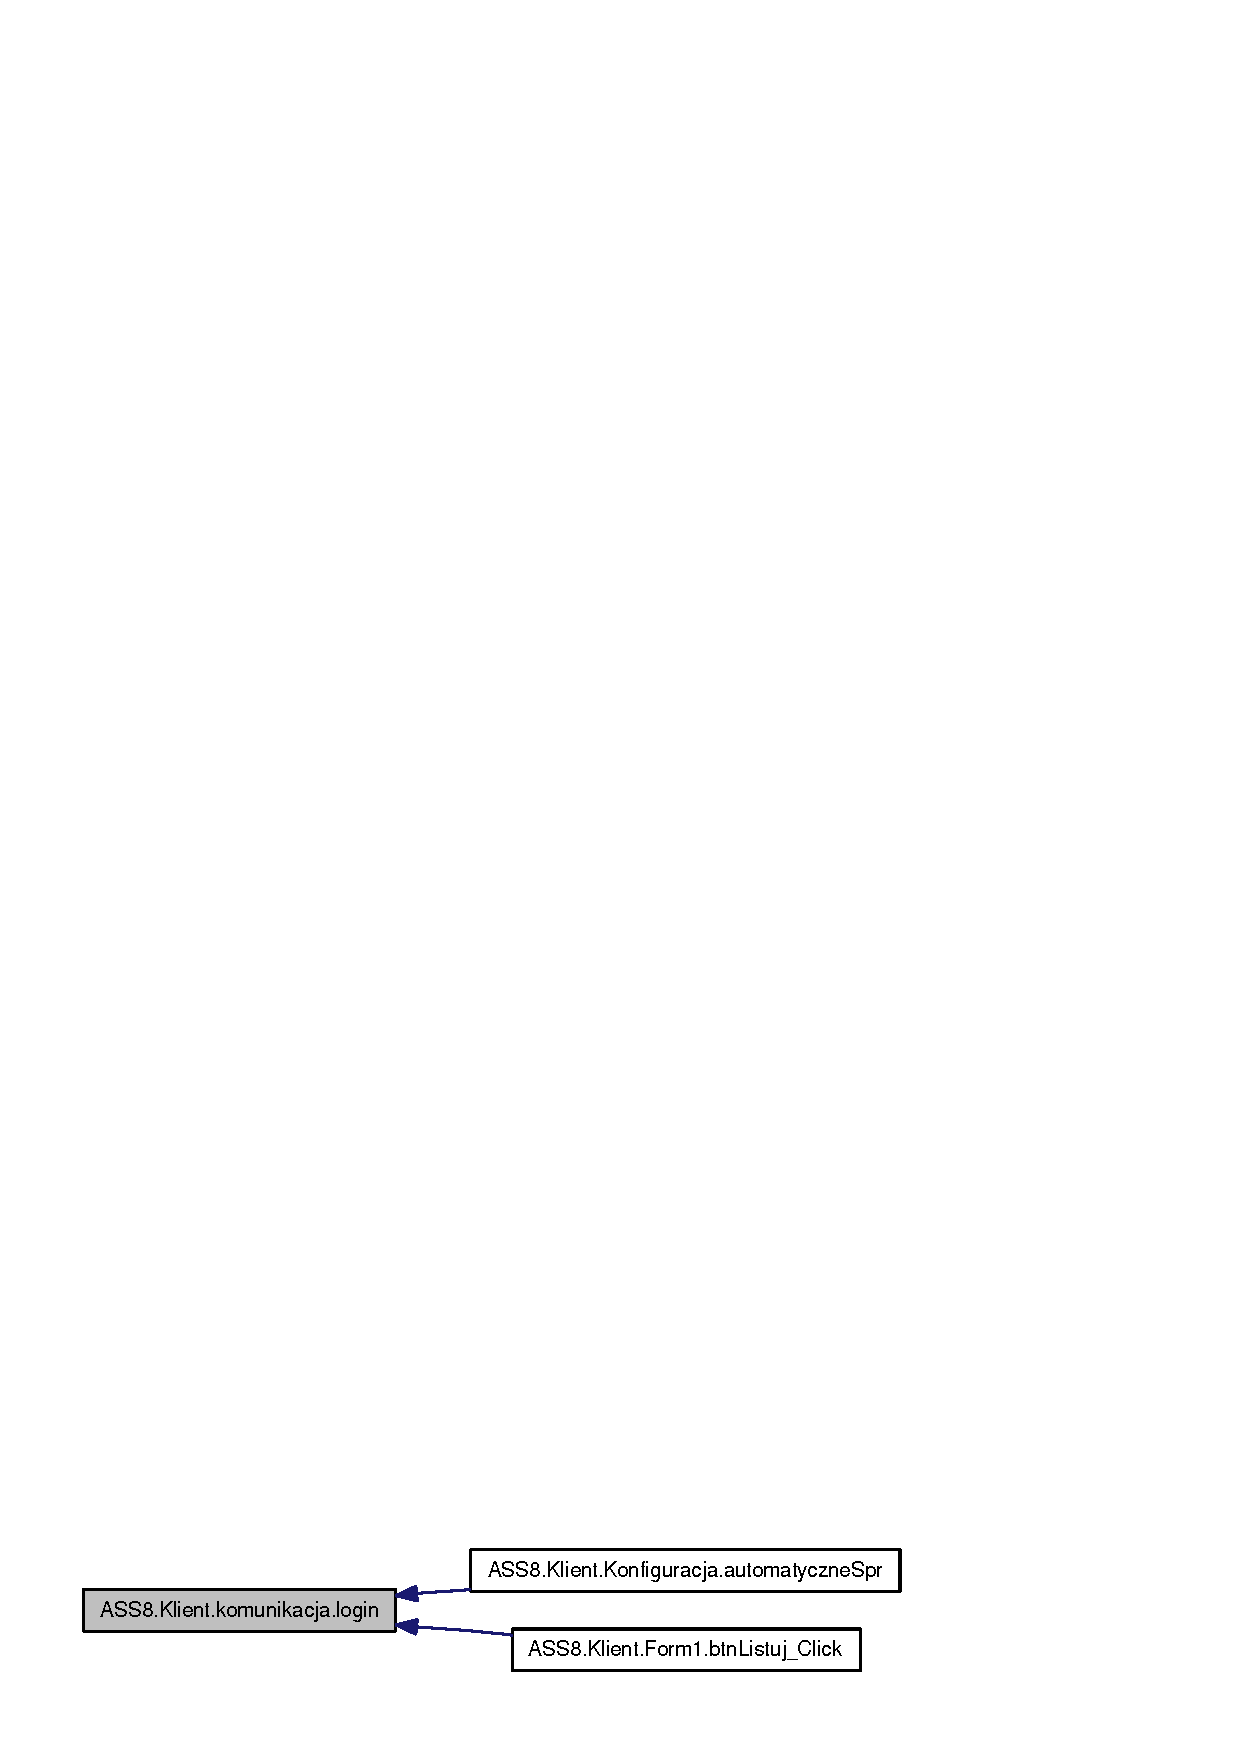
\includegraphics[width=218pt]{d7/dd4/a00013_cdc8379f1139bc25fb24a6c9b6ce1cc1_icgraph}
\end{center}
\end{figure}
\hypertarget{a00013_1b3c9442d102dd6e6b4d64cb0c31b660}{
\index{ASS8::Klient::komunikacja@{ASS8::Klient::komunikacja}!pobierz@{pobierz}}
\index{pobierz@{pobierz}!ASS8::Klient::komunikacja@{ASS8::Klient::komunikacja}}
\subsubsection[{pobierz}]{\setlength{\rightskip}{0pt plus 5cm}string ASS8.Klient.komunikacja.pobierz ()\hspace{0.3cm}{\tt  \mbox{[}private\mbox{]}}}}
\label{d7/dd4/a00013_1b3c9442d102dd6e6b4d64cb0c31b660}


Pobiera dane z serwera. 

\begin{Desc}
\item[Zwraca:]Wiadomość pobrana\end{Desc}


Definicja w linii 68 pliku komunikacja.cs.\hypertarget{a00013_19e1f9dd822287532839c60661237142}{
\index{ASS8::Klient::komunikacja@{ASS8::Klient::komunikacja}!pobierz@{pobierz}}
\index{pobierz@{pobierz}!ASS8::Klient::komunikacja@{ASS8::Klient::komunikacja}}
\subsubsection[{pobierz}]{\setlength{\rightskip}{0pt plus 5cm}int ASS8.Klient.komunikacja.pobierz (int {\em dlugosc}, \/  out byte\mbox{[}$\,$\mbox{]} {\em bytes})\hspace{0.3cm}{\tt  \mbox{[}private\mbox{]}}}}
\label{d7/dd4/a00013_19e1f9dd822287532839c60661237142}


Pobiera wiadomość od serwera. 

\begin{Desc}
\item[Parametry:]
\begin{description}
\item[{\em dlugosc}]Długość do pobrania\item[{\em bytes}]Tablica do zapisania odebranych danych\end{description}
\end{Desc}
\begin{Desc}
\item[Zwraca:]Długość faktycznie pobranych danych\end{Desc}


Definicja w linii 49 pliku komunikacja.cs.\hypertarget{a00013_2ff0f54013633857e608e3020ed82f70}{
\index{ASS8::Klient::komunikacja@{ASS8::Klient::komunikacja}!postep@{postep}}
\index{postep@{postep}!ASS8::Klient::komunikacja@{ASS8::Klient::komunikacja}}
\subsubsection[{postep}]{\setlength{\rightskip}{0pt plus 5cm}void ASS8.Klient.komunikacja.postep (ProgressBar {\em bar}, \/  int {\em progressValue})\hspace{0.3cm}{\tt  \mbox{[}private\mbox{]}}}}
\label{d7/dd4/a00013_2ff0f54013633857e608e3020ed82f70}


Aktualizuje postęp pliku w pasku postępu. 

\begin{Desc}
\item[Parametry:]
\begin{description}
\item[{\em bar}]Pasek postępu\item[{\em progressValue}]Wartość do zaktualizowania\end{description}
\end{Desc}


Definicja w linii 314 pliku komunikacja.cs.\hypertarget{a00013_5500d75da7421c54ebe1ab02e3386709}{
\index{ASS8::Klient::komunikacja@{ASS8::Klient::komunikacja}!ProgressBarHandler@{ProgressBarHandler}}
\index{ProgressBarHandler@{ProgressBarHandler}!ASS8::Klient::komunikacja@{ASS8::Klient::komunikacja}}
\subsubsection[{ProgressBarHandler}]{\setlength{\rightskip}{0pt plus 5cm}delegate void ASS8.Klient.komunikacja.ProgressBarHandler (ProgressBar {\em bar}, \/  int {\em progressValue})\hspace{0.3cm}{\tt  \mbox{[}private\mbox{]}}}}
\label{d7/dd4/a00013_5500d75da7421c54ebe1ab02e3386709}


\hypertarget{a00013_9449630c9b6bbf88144aba3981d8eb72}{
\index{ASS8::Klient::komunikacja@{ASS8::Klient::komunikacja}!uploadFile@{uploadFile}}
\index{uploadFile@{uploadFile}!ASS8::Klient::komunikacja@{ASS8::Klient::komunikacja}}
\subsubsection[{uploadFile}]{\setlength{\rightskip}{0pt plus 5cm}int ASS8.Klient.komunikacja.uploadFile (string {\em nazwa}, \/  DateTime {\em data}, \/  int {\em rozmiar})}}
\label{d7/dd4/a00013_9449630c9b6bbf88144aba3981d8eb72}


Wysyła plik na serwer. 

\begin{Desc}
\item[Parametry:]
\begin{description}
\item[{\em nazwa}]Nazwa pliku\item[{\em data}]Data pliku\item[{\em rozmiar}]Rozmiar pliku\end{description}
\end{Desc}
\begin{Desc}
\item[Zwraca:]Odpowiedź od serwera\end{Desc}


Definicja w linii 332 pliku komunikacja.cs.\hypertarget{a00013_da808f405d71a8f5f06659bac3b3fe50}{
\index{ASS8::Klient::komunikacja@{ASS8::Klient::komunikacja}!ustawUstawienia@{ustawUstawienia}}
\index{ustawUstawienia@{ustawUstawienia}!ASS8::Klient::komunikacja@{ASS8::Klient::komunikacja}}
\subsubsection[{ustawUstawienia}]{\setlength{\rightskip}{0pt plus 5cm}void ASS8.Klient.komunikacja.ustawUstawienia (string {\em s}, \/  int {\em p})}}
\label{d7/dd4/a00013_da808f405d71a8f5f06659bac3b3fe50}


Ustawia serwer i port do połączenia. 

\begin{Desc}
\item[Parametry:]
\begin{description}
\item[{\em s}]Adres serwera\item[{\em p}]Port serwera\end{description}
\end{Desc}


Definicja w linii 102 pliku komunikacja.cs.

Here is the caller graph for this function:\nopagebreak
\begin{figure}[H]
\begin{center}
\leavevmode
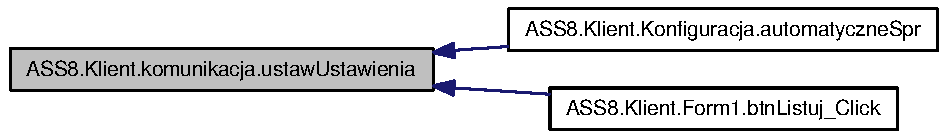
\includegraphics[width=245pt]{d7/dd4/a00013_da808f405d71a8f5f06659bac3b3fe50_icgraph}
\end{center}
\end{figure}
\hypertarget{a00013_302b89f984b2f9c695f1ae9462414d84}{
\index{ASS8::Klient::komunikacja@{ASS8::Klient::komunikacja}!usunPliki@{usunPliki}}
\index{usunPliki@{usunPliki}!ASS8::Klient::komunikacja@{ASS8::Klient::komunikacja}}
\subsubsection[{usunPliki}]{\setlength{\rightskip}{0pt plus 5cm}int ASS8.Klient.komunikacja.usunPliki (List$<$ {\bf pojedynczyPlik} $>$ {\em plikiDoUsuniecia})}}
\label{d7/dd4/a00013_302b89f984b2f9c695f1ae9462414d84}


Usuwa \hyperlink{a00017}{pliki} z serwer. 

\begin{Desc}
\item[Parametry:]
\begin{description}
\item[{\em plikiDoUsuniecia}]Lista plików do usunięcia\end{description}
\end{Desc}
\begin{Desc}
\item[Zwraca:]Odpowiedź od serwera\end{Desc}


Definicja w linii 518 pliku komunikacja.cs.\hypertarget{a00013_5069ee8ced0e023865e277f07ba690a9}{
\index{ASS8::Klient::komunikacja@{ASS8::Klient::komunikacja}!wyslij@{wyslij}}
\index{wyslij@{wyslij}!ASS8::Klient::komunikacja@{ASS8::Klient::komunikacja}}
\subsubsection[{wyslij}]{\setlength{\rightskip}{0pt plus 5cm}void ASS8.Klient.komunikacja.wyslij (byte\mbox{[}$\,$\mbox{]} {\em wiadomosc}, \/  int {\em dlugosc})}}
\label{d7/dd4/a00013_5069ee8ced0e023865e277f07ba690a9}


Wysyła wiadomość do serwera. 

\begin{Desc}
\item[Parametry:]
\begin{description}
\item[{\em wiadomosc}]Wiadomość do wysłania\item[{\em dlugosc}]Długość wiadomości\end{description}
\end{Desc}


Definicja w linii 31 pliku komunikacja.cs.

\subsection{Dokumentacja atrybutów składowych}
\hypertarget{a00013_2c01e8a98bfa8f0404b94af607eacbba}{
\index{ASS8::Klient::komunikacja@{ASS8::Klient::komunikacja}!endl@{endl}}
\index{endl@{endl}!ASS8::Klient::komunikacja@{ASS8::Klient::komunikacja}}
\subsubsection[{endl}]{\setlength{\rightskip}{0pt plus 5cm}const string {\bf ASS8.Klient.komunikacja.endl} = \char`\"{}$\backslash$r$\backslash$n$\backslash$r$\backslash$n\char`\"{}\hspace{0.3cm}{\tt  \mbox{[}private\mbox{]}}}}
\label{d7/dd4/a00013_2c01e8a98bfa8f0404b94af607eacbba}




Definicja w linii 23 pliku komunikacja.cs.\hypertarget{a00013_50e87371e5422a5bc0cb7b81a917e569}{
\index{ASS8::Klient::komunikacja@{ASS8::Klient::komunikacja}!endlOdp@{endlOdp}}
\index{endlOdp@{endlOdp}!ASS8::Klient::komunikacja@{ASS8::Klient::komunikacja}}
\subsubsection[{endlOdp}]{\setlength{\rightskip}{0pt plus 5cm}const string {\bf ASS8.Klient.komunikacja.endlOdp} = \char`\"{}\#\char`\"{}\hspace{0.3cm}{\tt  \mbox{[}private\mbox{]}}}}
\label{d7/dd4/a00013_50e87371e5422a5bc0cb7b81a917e569}




Definicja w linii 24 pliku komunikacja.cs.\hypertarget{a00013_1a50c04cee4acf979e3be6b7eeb41843}{
\index{ASS8::Klient::komunikacja@{ASS8::Klient::komunikacja}!folder@{folder}}
\index{folder@{folder}!ASS8::Klient::komunikacja@{ASS8::Klient::komunikacja}}
\subsubsection[{folder}]{\setlength{\rightskip}{0pt plus 5cm}string {\bf ASS8.Klient.komunikacja.folder}}}
\label{d7/dd4/a00013_1a50c04cee4acf979e3be6b7eeb41843}




Definicja w linii 90 pliku komunikacja.cs.\hypertarget{a00013_3003b01b9def7b324ad146f5598b00f1}{
\index{ASS8::Klient::komunikacja@{ASS8::Klient::komunikacja}!haslo@{haslo}}
\index{haslo@{haslo}!ASS8::Klient::komunikacja@{ASS8::Klient::komunikacja}}
\subsubsection[{haslo}]{\setlength{\rightskip}{0pt plus 5cm}string {\bf ASS8.Klient.komunikacja.haslo}\hspace{0.3cm}{\tt  \mbox{[}private\mbox{]}}}}
\label{d7/dd4/a00013_3003b01b9def7b324ad146f5598b00f1}




Definicja w linii 96 pliku komunikacja.cs.\hypertarget{a00013_4b00947de0ccf2197483dd77d35538f5}{
\index{ASS8::Klient::komunikacja@{ASS8::Klient::komunikacja}!log@{log}}
\index{log@{log}!ASS8::Klient::komunikacja@{ASS8::Klient::komunikacja}}
\subsubsection[{log}]{\setlength{\rightskip}{0pt plus 5cm}string {\bf ASS8.Klient.komunikacja.log}\hspace{0.3cm}{\tt  \mbox{[}private\mbox{]}}}}
\label{d7/dd4/a00013_4b00947de0ccf2197483dd77d35538f5}




Definicja w linii 95 pliku komunikacja.cs.\hypertarget{a00013_fad59850af421f7d3a2ad72f29fabe3d}{
\index{ASS8::Klient::komunikacja@{ASS8::Klient::komunikacja}!names@{names}}
\index{names@{names}!ASS8::Klient::komunikacja@{ASS8::Klient::komunikacja}}
\subsubsection[{names}]{\setlength{\rightskip}{0pt plus 5cm}XmlSerializerNamespaces {\bf ASS8.Klient.komunikacja.names}\hspace{0.3cm}{\tt  \mbox{[}private\mbox{]}}}}
\label{d7/dd4/a00013_fad59850af421f7d3a2ad72f29fabe3d}




Definicja w linii 91 pliku komunikacja.cs.\hypertarget{a00013_596f53c293d3811c950901c69c30aee4}{
\index{ASS8::Klient::komunikacja@{ASS8::Klient::komunikacja}!serverIP@{serverIP}}
\index{serverIP@{serverIP}!ASS8::Klient::komunikacja@{ASS8::Klient::komunikacja}}
\subsubsection[{serverIP}]{\setlength{\rightskip}{0pt plus 5cm}String {\bf ASS8.Klient.komunikacja.serverIP}\hspace{0.3cm}{\tt  \mbox{[}private\mbox{]}}}}
\label{d7/dd4/a00013_596f53c293d3811c950901c69c30aee4}




Definicja w linii 93 pliku komunikacja.cs.\hypertarget{a00013_6b37a2dd270fa5483aad7080a7ff71d4}{
\index{ASS8::Klient::komunikacja@{ASS8::Klient::komunikacja}!serverPort@{serverPort}}
\index{serverPort@{serverPort}!ASS8::Klient::komunikacja@{ASS8::Klient::komunikacja}}
\subsubsection[{serverPort}]{\setlength{\rightskip}{0pt plus 5cm}int {\bf ASS8.Klient.komunikacja.serverPort}\hspace{0.3cm}{\tt  \mbox{[}private\mbox{]}}}}
\label{d7/dd4/a00013_6b37a2dd270fa5483aad7080a7ff71d4}




Definicja w linii 94 pliku komunikacja.cs.\hypertarget{a00013_b992298af41161b42d77dbf23dfccad8}{
\index{ASS8::Klient::komunikacja@{ASS8::Klient::komunikacja}!sessionID@{sessionID}}
\index{sessionID@{sessionID}!ASS8::Klient::komunikacja@{ASS8::Klient::komunikacja}}
\subsubsection[{sessionID}]{\setlength{\rightskip}{0pt plus 5cm}int {\bf ASS8.Klient.komunikacja.sessionID}\hspace{0.3cm}{\tt  \mbox{[}private\mbox{]}}}}
\label{d7/dd4/a00013_b992298af41161b42d77dbf23dfccad8}




Definicja w linii 92 pliku komunikacja.cs.\hypertarget{a00013_d521d29af9bd410a982fb72814ae1eb0}{
\index{ASS8::Klient::komunikacja@{ASS8::Klient::komunikacja}!socket@{socket}}
\index{socket@{socket}!ASS8::Klient::komunikacja@{ASS8::Klient::komunikacja}}
\subsubsection[{socket}]{\setlength{\rightskip}{0pt plus 5cm}Socket {\bf ASS8.Klient.komunikacja.socket}\hspace{0.3cm}{\tt  \mbox{[}private\mbox{]}}}}
\label{d7/dd4/a00013_d521d29af9bd410a982fb72814ae1eb0}




Definicja w linii 25 pliku komunikacja.cs.

\subsection{Dokumentacja właściwości}
\hypertarget{a00013_3c5917b1f8a0fb187d3c48ff22b25ec6}{
\index{ASS8::Klient::komunikacja@{ASS8::Klient::komunikacja}!Haslo@{Haslo}}
\index{Haslo@{Haslo}!ASS8::Klient::komunikacja@{ASS8::Klient::komunikacja}}
\subsubsection[{Haslo}]{\setlength{\rightskip}{0pt plus 5cm}string ASS8.Klient.komunikacja.Haslo\hspace{0.3cm}{\tt  \mbox{[}get, set\mbox{]}}}}
\label{d7/dd4/a00013_3c5917b1f8a0fb187d3c48ff22b25ec6}


Właściwość ustawia lub zwraca hasło do połączenia z serwerem. 



Definicja w linii 596 pliku komunikacja.cs.\hypertarget{a00013_2c321eee82dba3f82cae18a5b4d6d620}{
\index{ASS8::Klient::komunikacja@{ASS8::Klient::komunikacja}!Login@{Login}}
\index{Login@{Login}!ASS8::Klient::komunikacja@{ASS8::Klient::komunikacja}}
\subsubsection[{Login}]{\setlength{\rightskip}{0pt plus 5cm}string ASS8.Klient.komunikacja.Login\hspace{0.3cm}{\tt  \mbox{[}get, set\mbox{]}}}}
\label{d7/dd4/a00013_2c321eee82dba3f82cae18a5b4d6d620}


Właściwość ustawia lub zwraca login do połączenia z serwerem. 



Definicja w linii 562 pliku komunikacja.cs.\hypertarget{a00013_90c9595c1609fb8364d7e2a8d806a27c}{
\index{ASS8::Klient::komunikacja@{ASS8::Klient::komunikacja}!Port@{Port}}
\index{Port@{Port}!ASS8::Klient::komunikacja@{ASS8::Klient::komunikacja}}
\subsubsection[{Port}]{\setlength{\rightskip}{0pt plus 5cm}int ASS8.Klient.komunikacja.Port\hspace{0.3cm}{\tt  \mbox{[}get\mbox{]}}}}
\label{d7/dd4/a00013_90c9595c1609fb8364d7e2a8d806a27c}


Właściwość ustawia lub zwraca port do połączenia z serwerem. 



Definicja w linii 586 pliku komunikacja.cs.\hypertarget{a00013_d9eb3fc56fa999cc46116e3d7019f070}{
\index{ASS8::Klient::komunikacja@{ASS8::Klient::komunikacja}!Serwer@{Serwer}}
\index{Serwer@{Serwer}!ASS8::Klient::komunikacja@{ASS8::Klient::komunikacja}}
\subsubsection[{Serwer}]{\setlength{\rightskip}{0pt plus 5cm}string ASS8.Klient.komunikacja.Serwer\hspace{0.3cm}{\tt  \mbox{[}get\mbox{]}}}}
\label{d7/dd4/a00013_d9eb3fc56fa999cc46116e3d7019f070}


Właściwość ustawia lub zwraca adres do połączenia z serwerem. 



Definicja w linii 576 pliku komunikacja.cs.

Dokumentacja dla tej klasy została wygenerowana z pliku:\begin{CompactItemize}
\item 
\hyperlink{a00049}{komunikacja.cs}\end{CompactItemize}
